\documentclass{article}
\usepackage[a4paper, margin=20mm]{geometry}
\usepackage{graphicx}
\usepackage{float}
\usepackage{amsmath}
\usepackage{amsfonts}
\usepackage{caption}
\usepackage{subcaption}

\title{Practical Submission Sheet}
\newcommand{\bb}[1]{\textbf{#1}}
%\newcommand{\it}[1]{\textit{#1}}
\newcommand{\ol}[1]{\overline{#1}}
\date{}
\begin{document}
	\maketitle
	
	\hrulefill
	\begin{center}
		\begin{tabular}{lll}
			\textit{Term}: 2020-1 & & \hfill \textit{Submission Date}: \today\\
			\textit{Lecture Date}: October 30, 2020. & & \textit{Practical Number}: 10\\
			\textit{Course Code}: PHY249 & & \textit{Section}: G2903\\
			\textit{Registration Number}: 11912610 & & \textit{Roll No}: 03\\
			\textit{Student Name}: Aayush Arya & & \\
		\end{tabular}
	\end{center}
	
	\hrulefill
	
	\section*{Aim} To design half-subtractor, full subtractor and 4-bit binary subtractor circuits using any gate combination.
	
	\section*{Concepts Learnt}	
	Learnt how to implement half subtractor, and full subtractor circuits, including those for 4-bit binary numbers (4-bit binary subtractor.)
	
	\section*{Key Observations \& Insights}
	The truth tables for all the circuits were verified. The boolean expressions for difference and borrow of half adder are $D = A \oplus B $ and $C = \overline{A}\cdot B$. For full subtractor, they are $D = (A \oplus B) \oplus B_{in}$ and $B_{out} = \overline{A}\cdot B + \overline{(A\oplus B)}\cdot B_{in}$
	
	\section*{Application Areas}
	Binary operations are ubiquitous in digital electronics. Thus, it's essential to know how to design a circuit that can perform binary subtraction operations on single or multi-bit numbers.
	
	\section*{Report}
	
	A half-subtractor circuit can be used to subtract two single bit numbers. The rules for binary subtraction $D = A-B$ give us logic functions for difference and borrow in binary subtraction $D = A \oplus B$ and $B_{out} = \overline{A}\cdot B$ respectively.\\
	
	The truth table for these output functions is then
	\begin{table}[H]
		\centering
		\begin{tabular}{|c|c|c|c|}
			\hline
			Input A & Input B & Difference (D) & Borrow (B$_{out}$)\\
			\hline
			0 & 0 & 0 & 0\\
			0 & 1 & 1 & 1\\
			1 & 0 & 1 & 0\\
			1 & 1 & 0 & 0\\
			\hline
		\end{tabular}
		\caption{Truth table for half-subtractor circuit.}
	\end{table}
	
	\begin{figure}[H]
		\centering
		\begin{subfigure}[t]{0.4\textwidth}
			\centering
			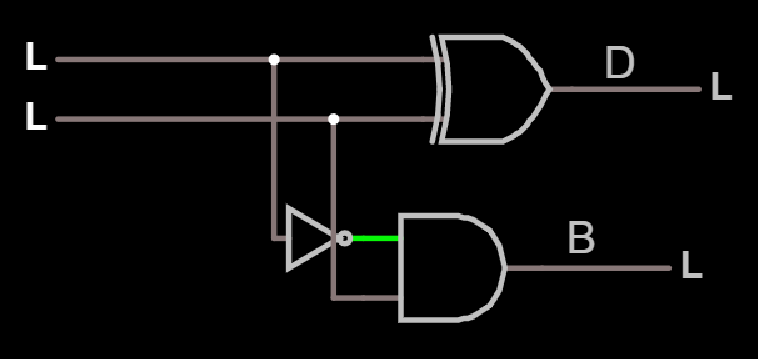
\includegraphics[width=\textwidth]{half_sub/half_sub_00.png}
			\caption{$A=0, B=0$}
		\end{subfigure}
		\begin{subfigure}[t]{.4\textwidth}
			\centering
			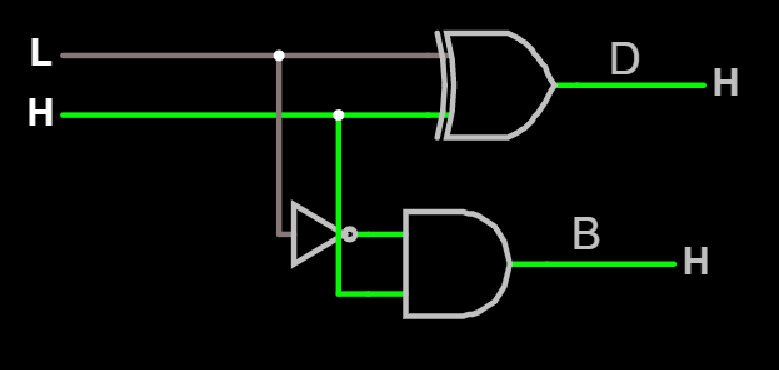
\includegraphics[width=\textwidth]{half_sub/half_sub_01.png}
			\caption{$A=0, B=1$}
		\end{subfigure}
		
		\begin{subfigure}[b]{0.4\textwidth}
			\centering
			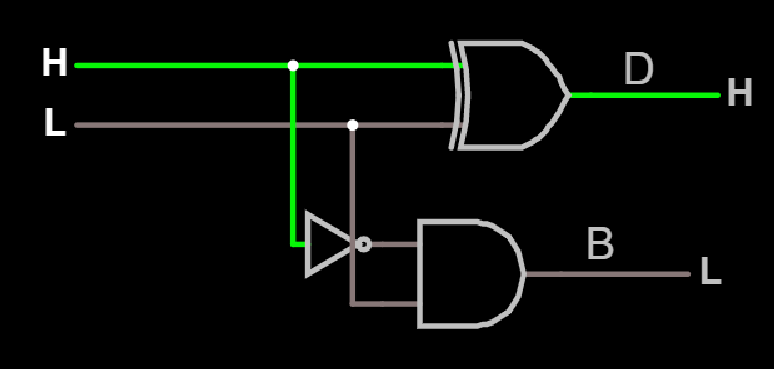
\includegraphics[width=\textwidth]{half_sub/half_sub_10.png}
			\caption{$A=1, B=0$}
		\end{subfigure}
		\begin{subfigure}[b]{0.4\textwidth}
			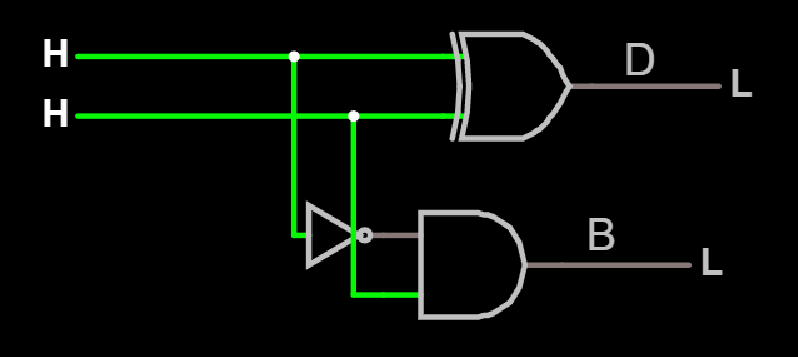
\includegraphics[width=\textwidth]{half_sub/half_sub_11.png}
			\caption{$A=1, B=1$}
		\end{subfigure}
		\caption{Different output states for a half-subtractor circuit}
		\label{fig:halfsub}
	\end{figure}
	
	A half subtractor, however, is insufficient for handling binary numbers of more than one bit. For that purpose, a \textit{full subtractor} circuit is used.
	
	Difference and borrow for it are defined as $$D = (A \oplus B) \oplus B_{in}$$ and $$B_{out} = \overline{A}\cdot B + \overline{(A\oplus B)}\cdot B_{in}$$
	
	The truth table for this set of logic functions is.
	\begin{table}[H]
		\centering
		\begin{tabular}{|c|c|c|c|c|}
			\hline
			Input A & Input B & B$_{in}$ & Difference (D) & Borrow (B$_{out}$)\\
			\hline 
			0 & 0 & 0 & 0 & 0\\
			0 & 1 & 0 & 1 & 0\\
			1 & 0 & 0 & 1 & 0\\
			1 & 1 & 0 & 0 & 1\\
			\hline
			0 & 0 & 1 & 1 & 0\\
			0 & 1 & 1 & 0 & 1\\
			1 & 0 & 1 & 0 & 1\\
			1 & 1 & 1 & 1 & 1\\
			\hline
		\end{tabular}
		\caption{Truth table for full adder.}
	\end{table}
	
	The circuit for a full subtractor was constructed based on the boolean expressions for $D$ and $B_{out}$ and its different states are shown in Figure 2.
	
	\begin{figure}[H]
		\centering
		\begin{subfigure}[t]{0.4\textwidth}
			\centering
			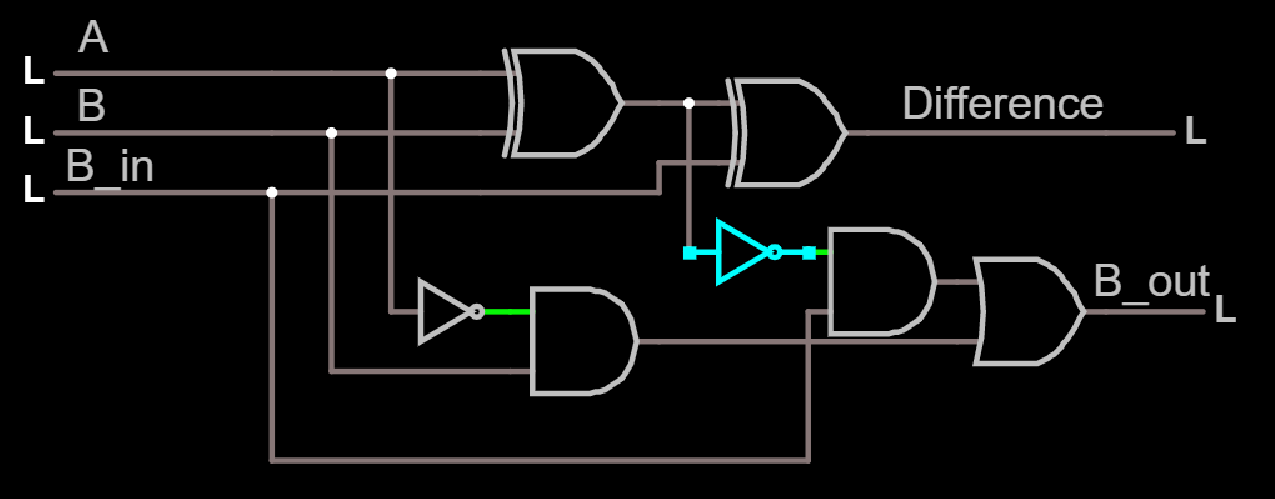
\includegraphics[width=\textwidth]{full_sub/full_sub_000.png}
		\end{subfigure}
		\begin{subfigure}[t]{.4\textwidth}
			\centering
			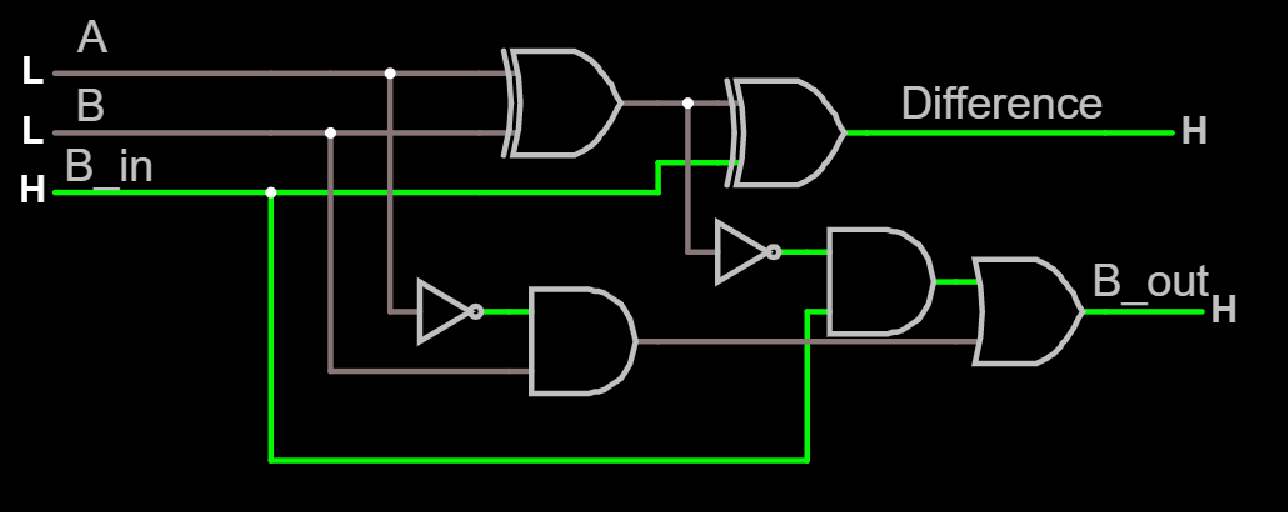
\includegraphics[width=\textwidth]{full_sub/full_sub_001.png}
		\end{subfigure}
		
		\begin{subfigure}[b]{0.4\textwidth}
			\centering
			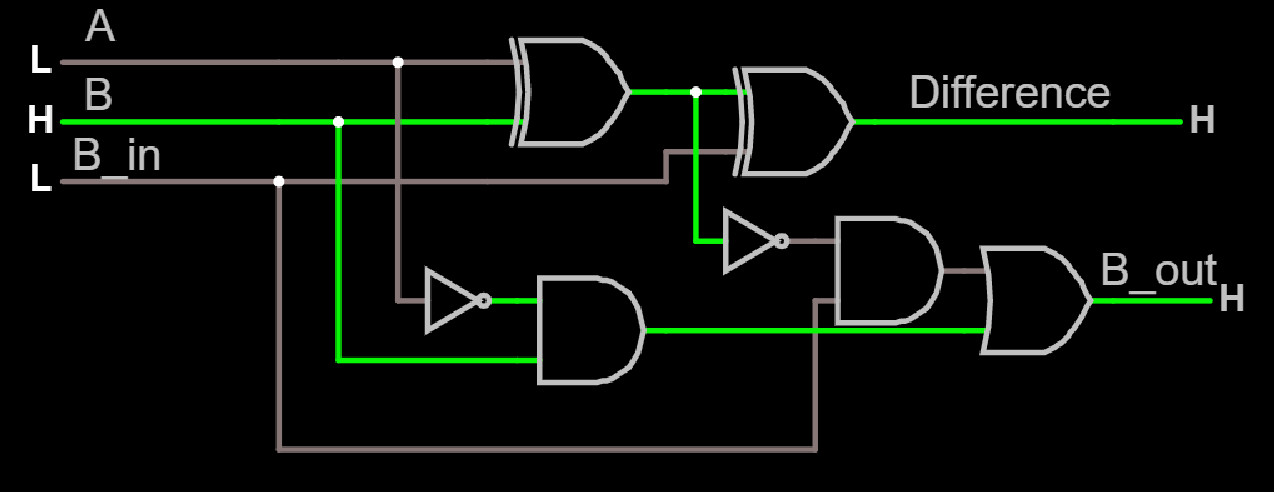
\includegraphics[width=\textwidth]{full_sub/full_sub_010.png}
		\end{subfigure}
		\begin{subfigure}[b]{0.4\textwidth}
			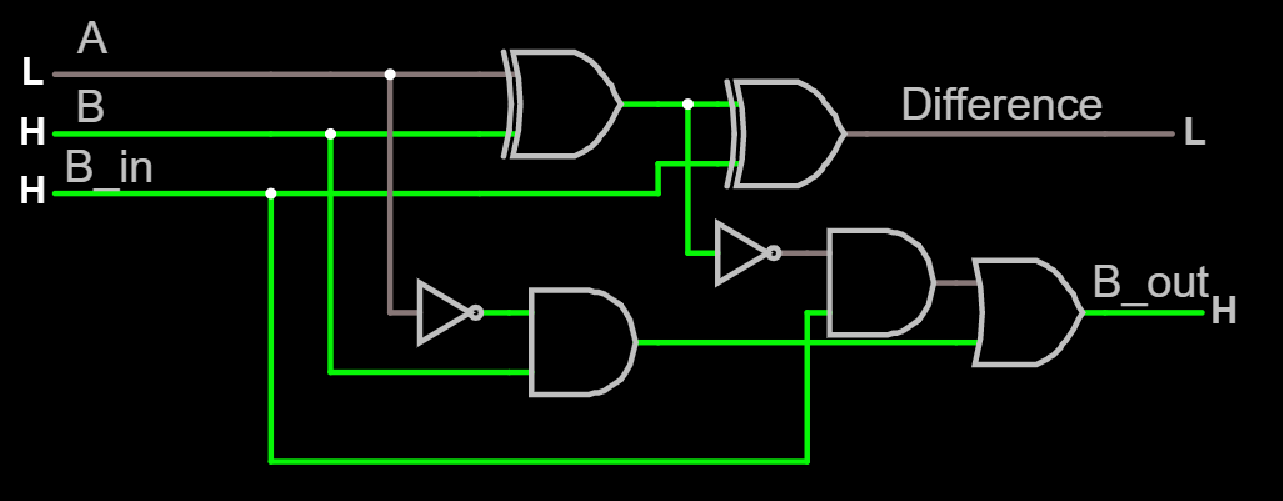
\includegraphics[width=\textwidth]{full_sub/full_sub_011.png}
		\end{subfigure}
		
		\begin{subfigure}[b]{0.4\textwidth}
			\centering
			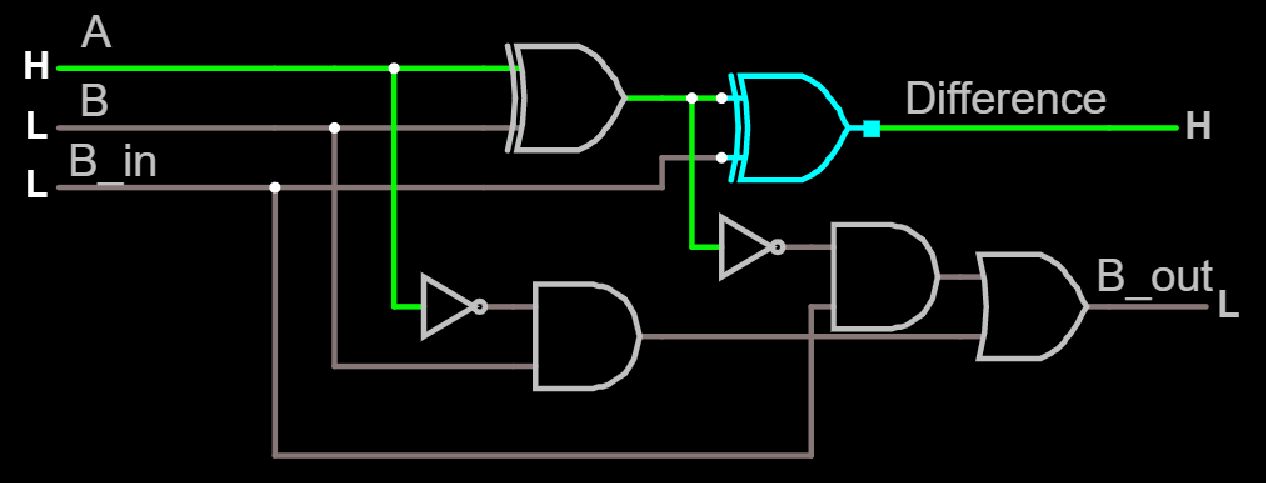
\includegraphics[width=\textwidth]{full_sub/full_sub_100.png}
		\end{subfigure}
		\begin{subfigure}[b]{0.4\textwidth}
			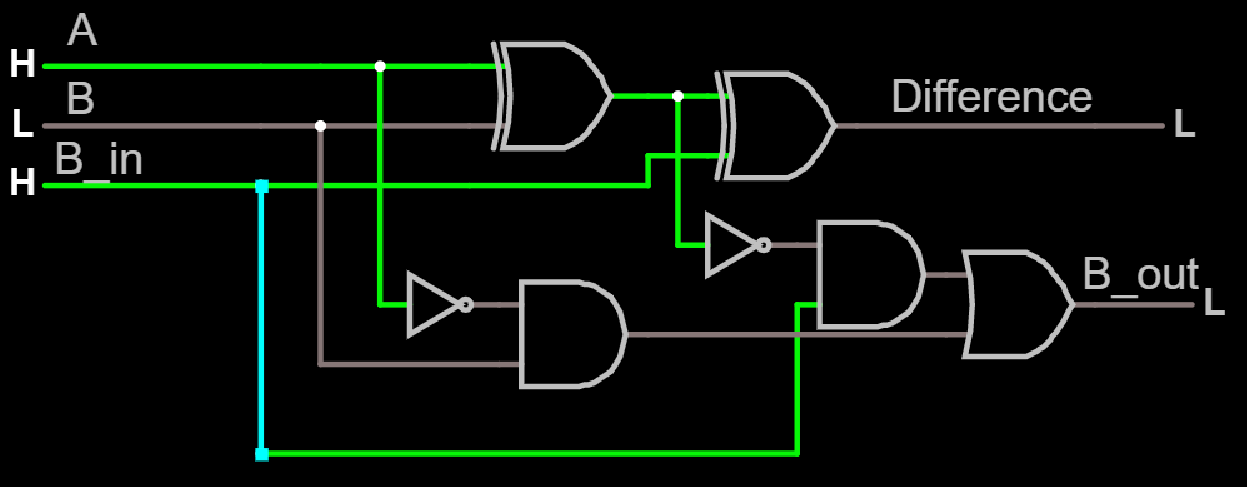
\includegraphics[width=\textwidth]{full_sub/full_sub_101.png}
		\end{subfigure}
		
		\begin{subfigure}[b]{0.4\textwidth}
			\centering
			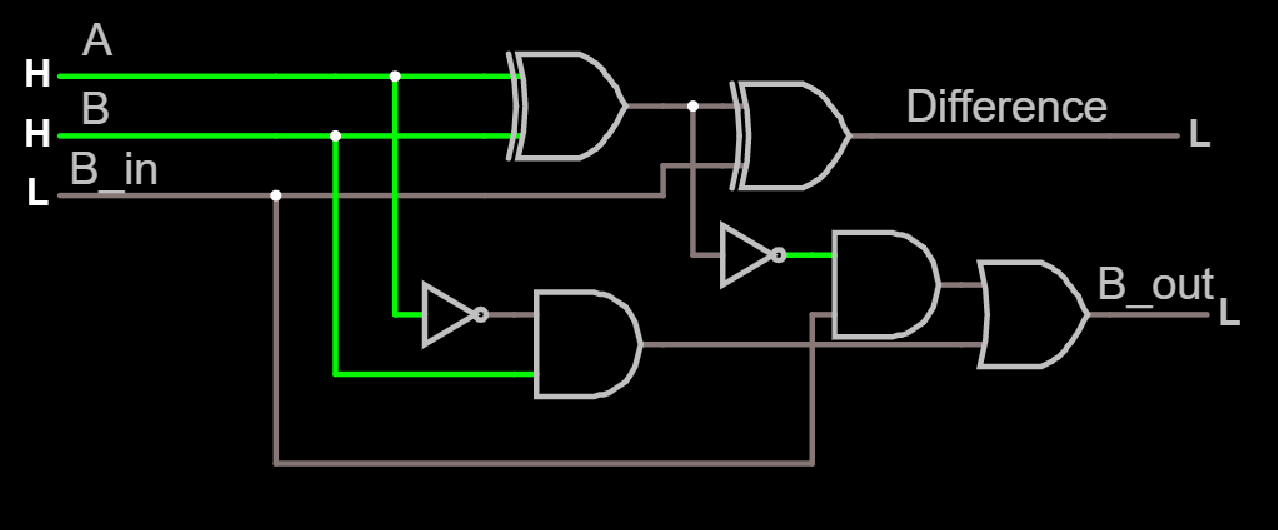
\includegraphics[width=\textwidth]{full_sub/full_sub_110.png}
		\end{subfigure}
		\begin{subfigure}[b]{0.4\textwidth}
			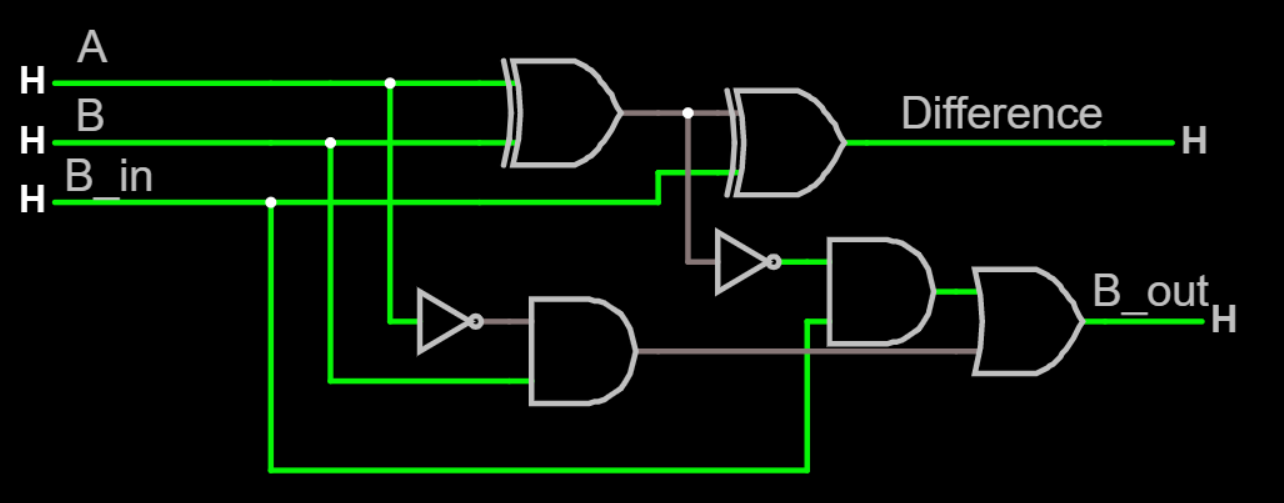
\includegraphics[width=\textwidth]{full_sub/full_sub_111.png}
		\end{subfigure}
		\caption{Different output states for a full-subtractor circuit}
		\label{fig:fulladder}
	\end{figure}
	
	Using combinations of full subtractor circuits, subtractors of multi-bit numbers can be constructed. The construction for 4 bit binary subtractor and its different outputs for different inputs are shown in Figures 3 and 4.\\

	The result of subtraction of two binary numbers $X_4X_3X_2X_1$ and $Y_4Y_3Y_2Y_1$ is $D_4D_3D_2D_1$. In Figures 3-4, the digits $X_4$, .. $X_1$ and $Y_4$, .. $Y_1$ are inputs to the full subtractors and $D_1$, .. $D_4$ are received as outputs of the "difference" function.
	\begin{figure}[H]
		\centering
		\begin{subfigure}[t]{0.8\textwidth}
			\centering
			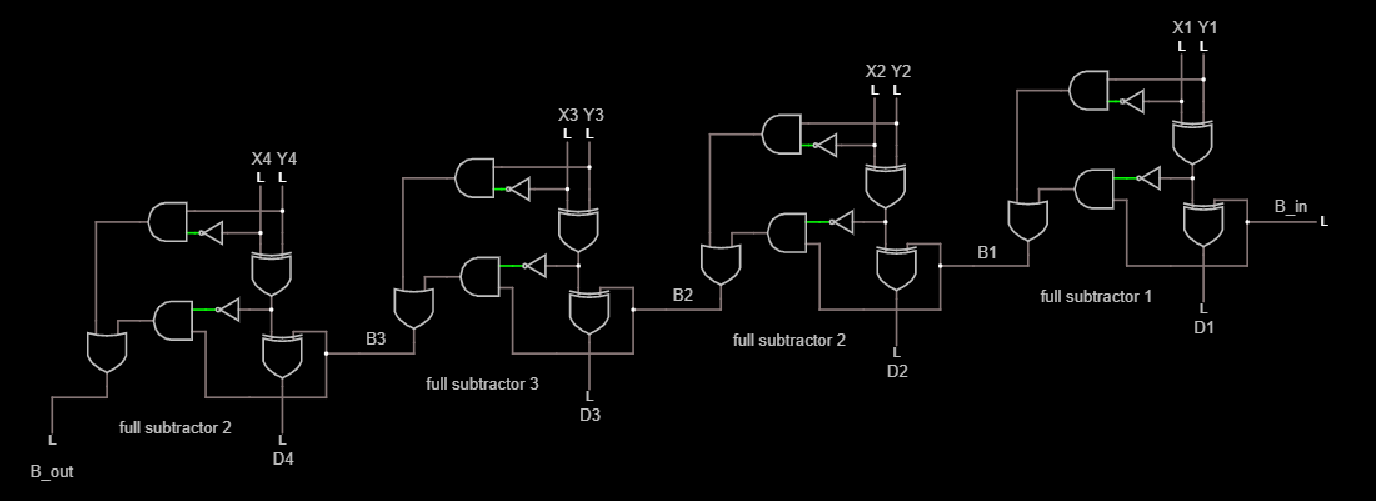
\includegraphics[width=\textwidth]{4bit/4bit_000.png}
		\end{subfigure}
		
		\begin{subfigure}[b]{0.8\textwidth}
			\centering
			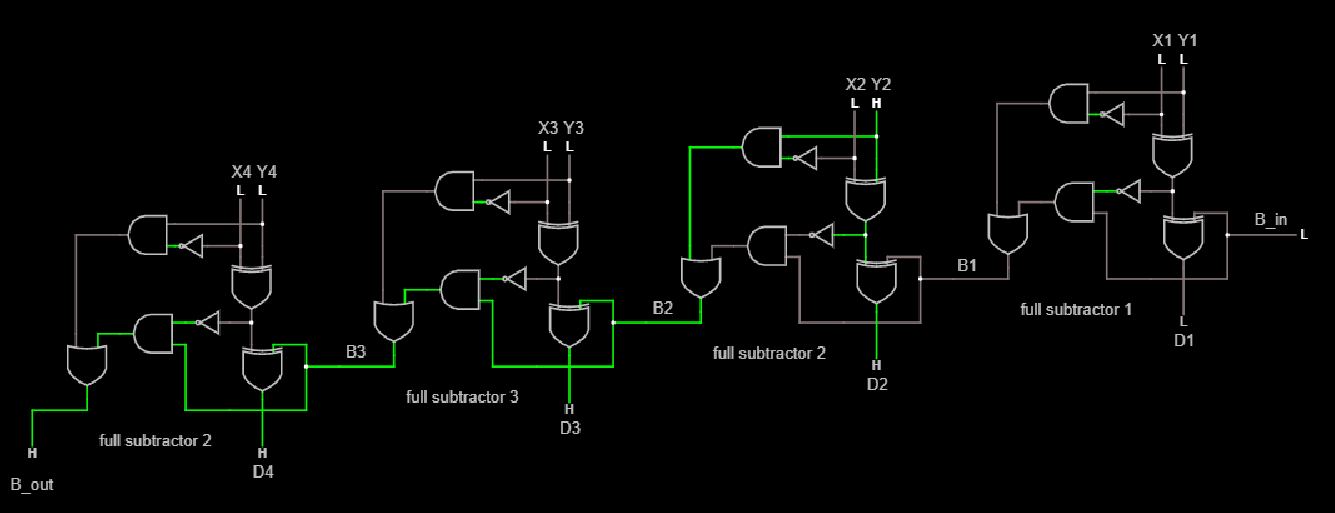
\includegraphics[width=\textwidth]{4bit/4bit_010.png}
		\end{subfigure}
		
		\begin{subfigure}[b]{0.8\textwidth}
			\centering
			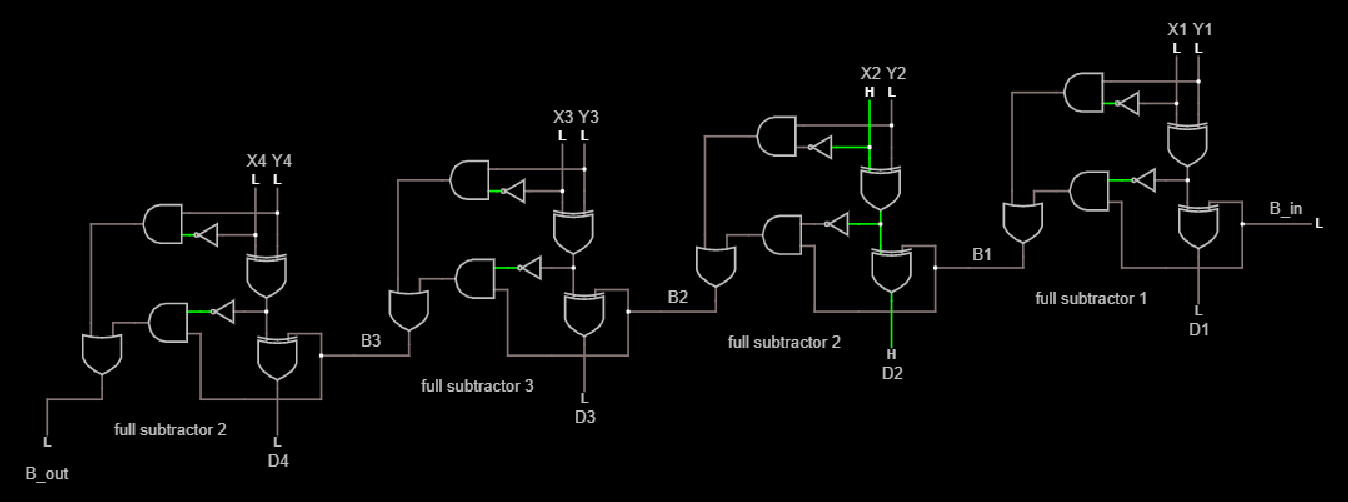
\includegraphics[width=\textwidth]{4bit/4bit_100.png}
		\end{subfigure}
		
		\begin{subfigure}[b]{0.8\textwidth}
			\centering
			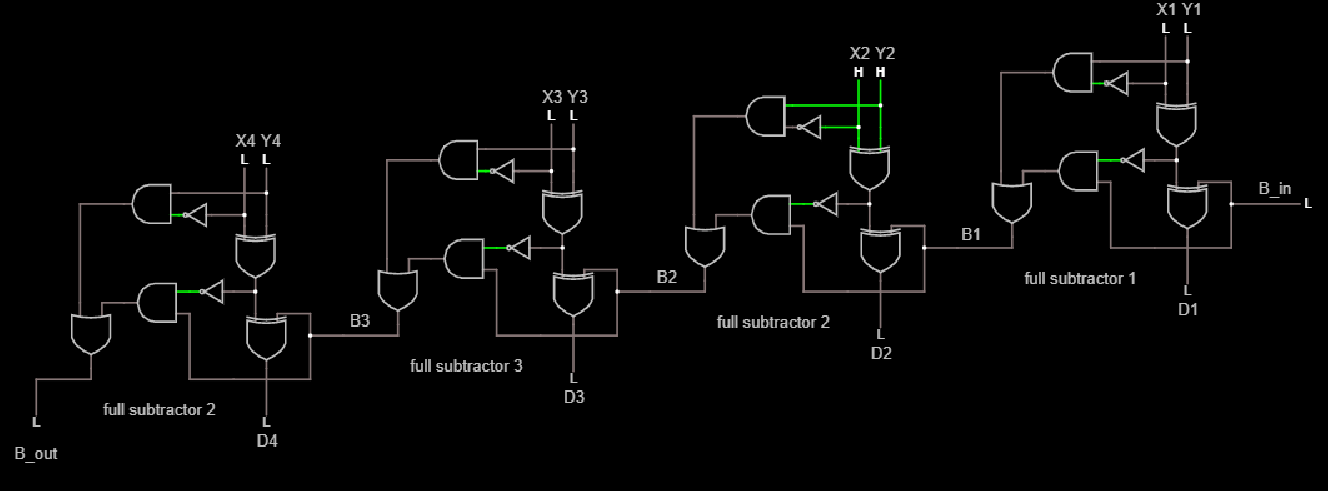
\includegraphics[width=\textwidth]{4bit/4bit_110.png}
		\end{subfigure}
		
		\caption{4-bit subtractor circuit}
		\label{4bit1}
	\end{figure}
	
	
	\begin{figure}
		\centering
		
		\begin{subfigure}[t]{.8\textwidth}
			\centering
			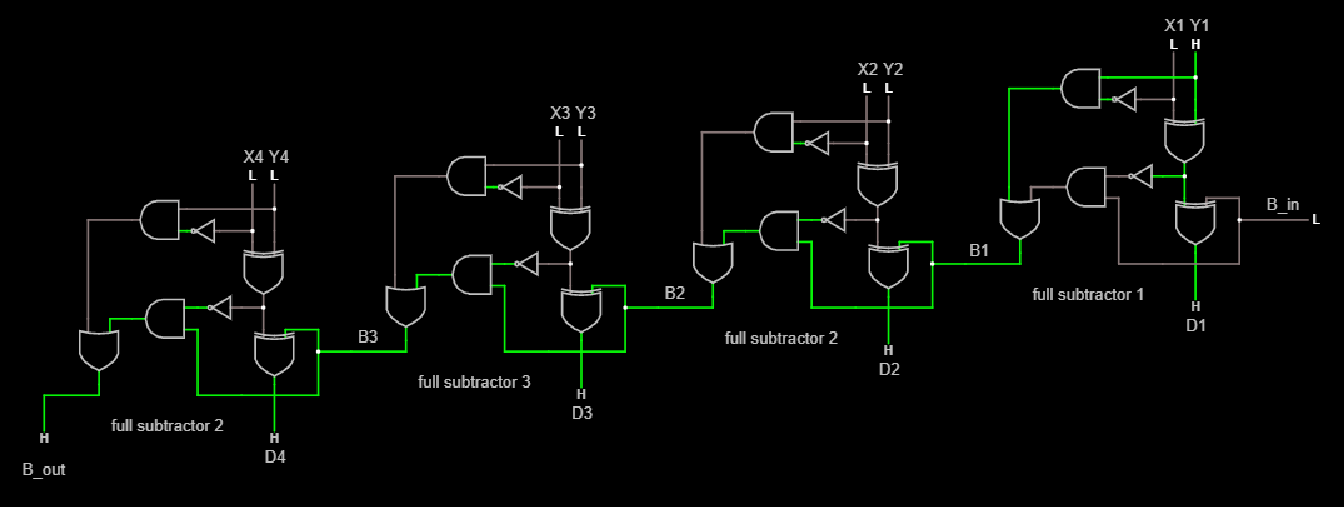
\includegraphics[width=\textwidth]{4bit/4bit_001.png}
		\end{subfigure}
		
		\begin{subfigure}[b]{0.8\textwidth}
			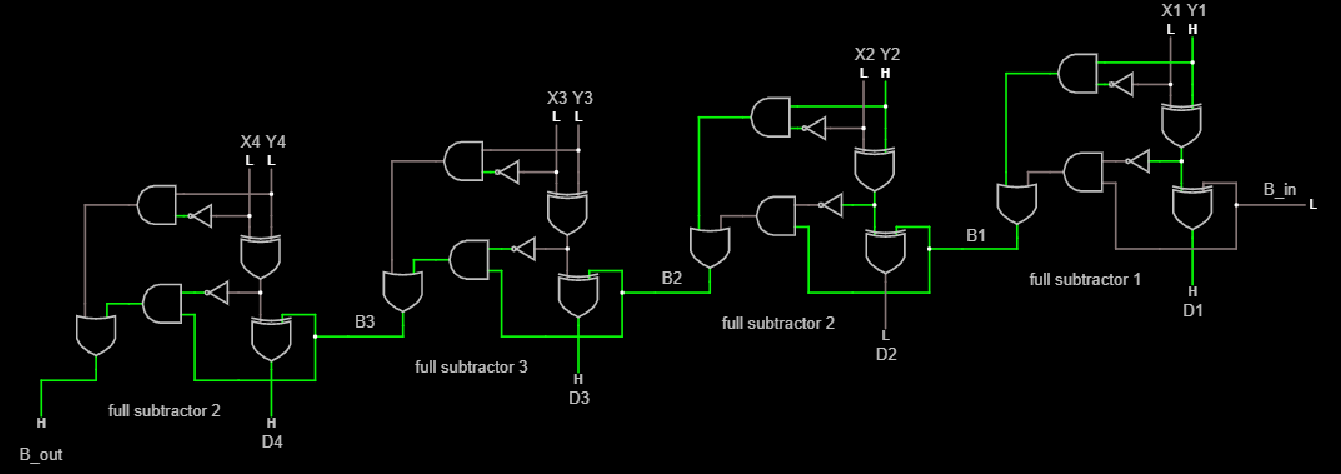
\includegraphics[width=\textwidth]{4bit/4bit_011.png}
		\end{subfigure}
		
		\begin{subfigure}[b]{0.8\textwidth}
			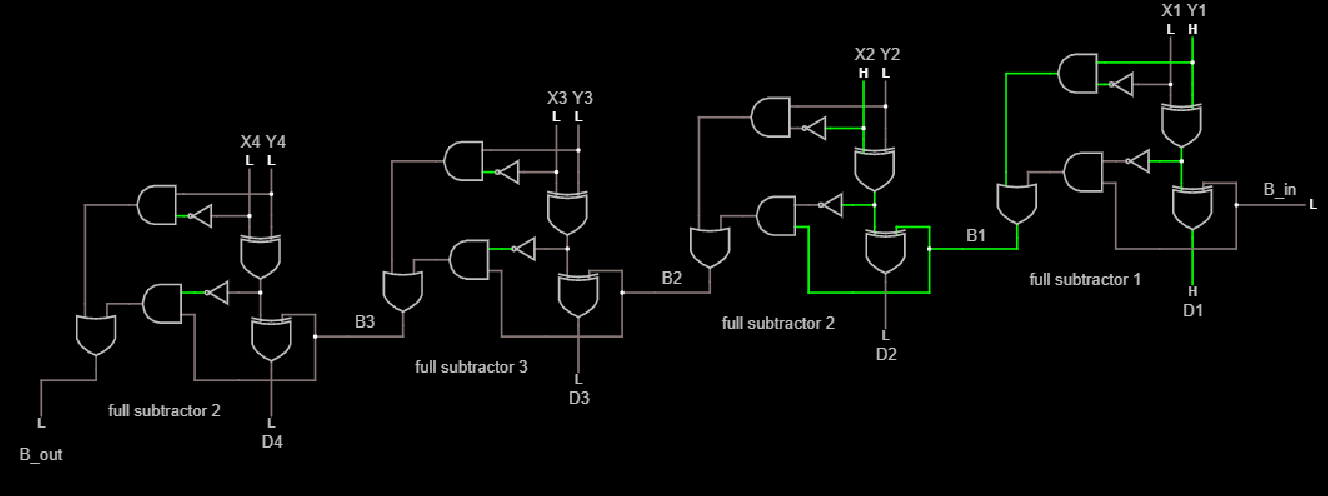
\includegraphics[width=\textwidth]{4bit/4bit_101.png}
		\end{subfigure}
		
		\begin{subfigure}[b]{0.8\textwidth}
			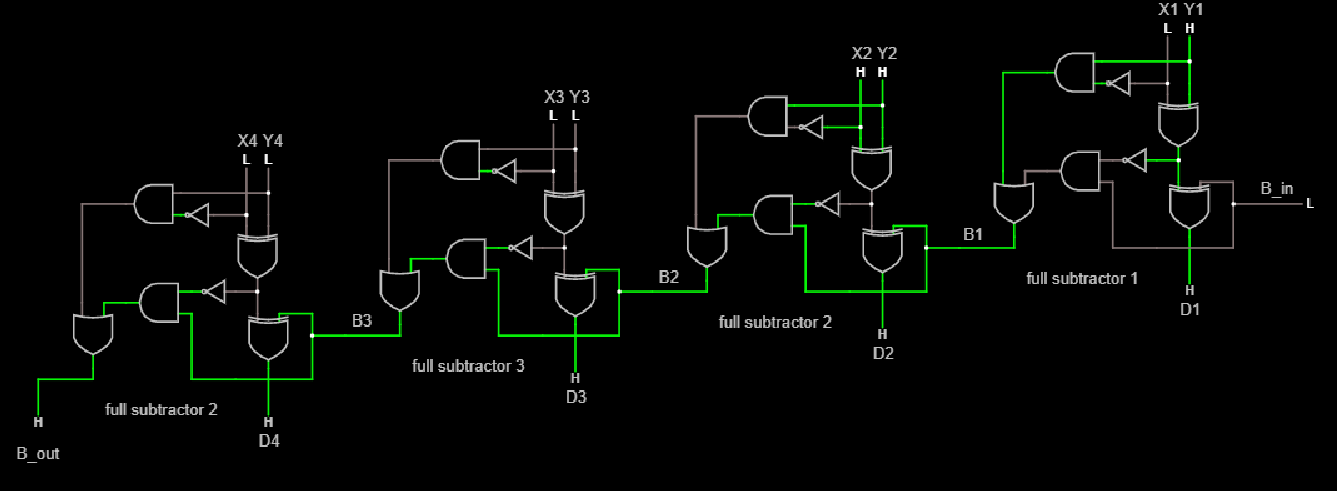
\includegraphics[width=\textwidth]{4bit/4bit_111.png}
		\end{subfigure}
		\caption{(Cont.) 4-bit subtractor circuit.}
		\label{4bit2}
	\end{figure}
\end{document}